\section{Results}

An initial goal of this project was to create a model of my head for 3d printing,
but it was difficult to keep a consistent posture for multiple angles.

\begin{figure}[h]
\centering
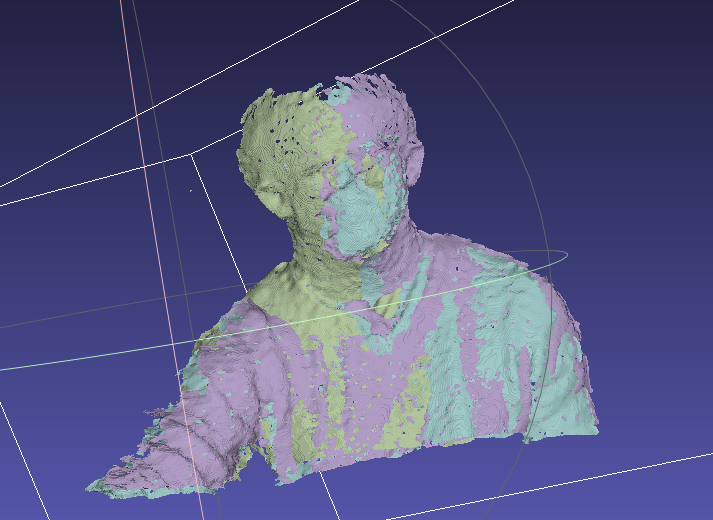
\includegraphics[width=0.6\textwidth]{poor_alignment.png}
\caption{Difficult to take depth selfies from different angles without moving}
\end{figure}

Photography skill (and a longer USB cable!) would be helpful for capturing quality depth images.
When the object is not rigid across different frames the point clouds do not quite fit together.

For the Cube Man project, the final reconstructions are somewhat disappointing.
None of the reconstruction methods tried generate a smooth and detailed model.
Even after carefully aligning multiple clouds the reconstruction obtained
from the merged point clouds is jagged and full of artifacts.

\begin{figure}[H]
\centering
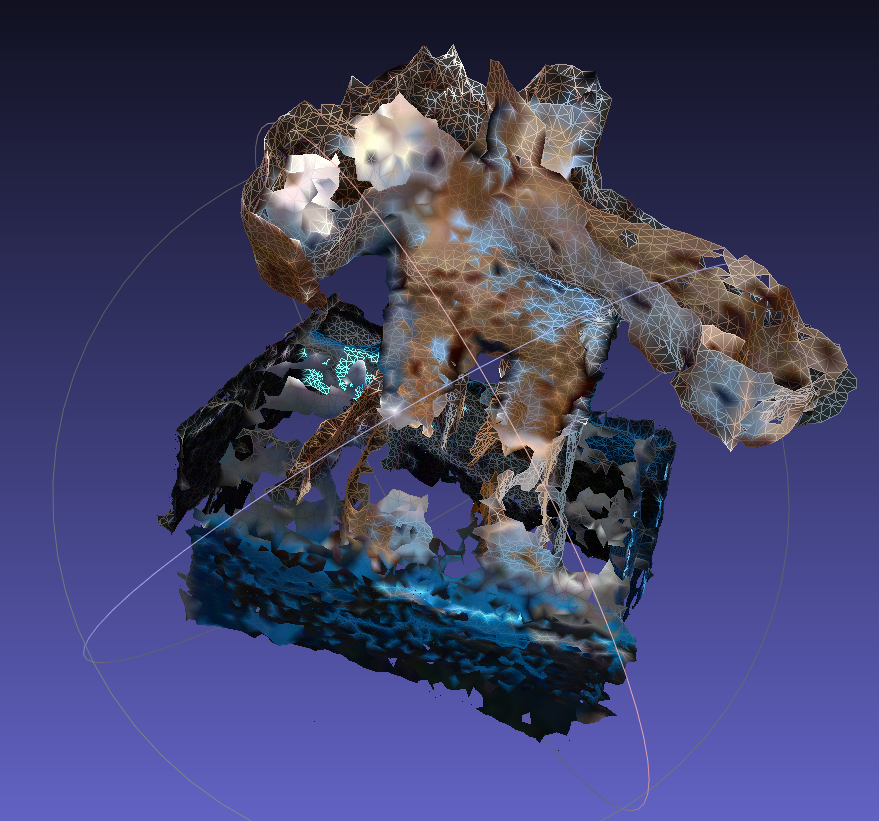
\includegraphics[width=0.6\textwidth]{simplified_point_cloud_ball_pivot_reconstruction.png}
\caption{Reconstruction with Ball Pivot Method from Simplified Point Cloud }
\end{figure}


\begin{figure}[H]
\centering
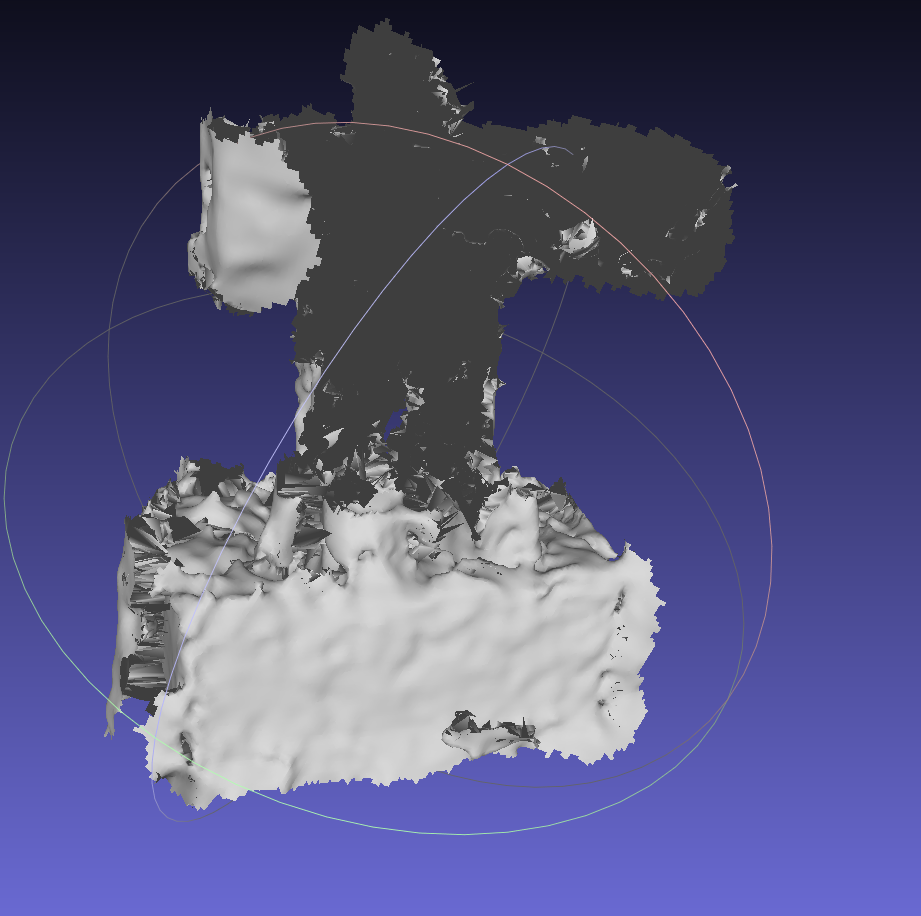
\includegraphics[width=0.6\textwidth]{simplified_point_cloud_marching_cubes.png}
\caption{Reconstruction with Marching Cubes from Simplified Point Cloud }
\end{figure}

The reality is that these devices may not have sufficient accuracy at small scales.
The infrared emitter mitigates some of the problems of stereoscopic depth but
also seems to introduce some noise.

With Fusion and variants, errors are mitigated using big data approaches to identify noise,
discard erroneous values and fill in holes and details. It seems probable that a Fusion method \cite{newcombe2011kinectfusion}
 would provide better results than this artisanal approach.

The D435 is perhaps better suited for sparse Simultaneous Location and Mapping, real-time background subtraction and other applications that do not require fine detail, only a general outline of
surfaces (like Fruit Ninja and similar games).
